\documentclass[11pt, oneside]{article}
\usepackage[letterpaper, margin=2cm]{geometry}
\usepackage{MATH667}
\usepackage{booktabs}

\begin{document}
\noindent \textbf{\Large{Caleb Logemann \\
MATH667 Hyperbolic Partial Differential Equations \\
Homework 6
}}

%\lstinputlisting[language=MATLAB]{H01_23.m}
\begin{enumerate}
  \item % #1
    \begin{enumerate}
      \item[(a)]
        The following are my methods for the second order Upwind, Central and
        MUSCL schemes.
        The main difference in these functions is the different definitions of
        the numerical flux.
        \lstinputlisting[language=MATLAB]{upwindFV2.m}
        \lstinputlisting[language=MATLAB]{centralFV2.m}
        \lstinputlisting[language=MATLAB]{muscl2.m}

        The following script now performs a test for the order of accuracy of
        these three methods.
        \lstinputlisting[language=MATLAB, lastline=41]{H06.m}
        Note that I am using the forward Euler timestepping, so the methods
        should only achieve first order accuracy even though the methods are
        second order in space.

        \begin{center}
          Central Scheme \\
          \begin{tabular}{*{5}{c}}
            \toprule
            N & $\Delta x$ & $L^{\infty}$ Error & Order \\
            \midrule
            20 & 0.314 & 0.075 & - \\
            40 & 0.157 & 0.035 & 1.103 \\
            80 & 0.079 & 0.017 & 1.059 \\
            160 & 0.039 & 0.008 & 1.085 \\
            \bottomrule
          \end{tabular}
        \end{center}

        \begin{center}
          Upwind Scheme \\
          \begin{tabular}{*{5}{c}}
            \toprule
            N & $\Delta x$ & $L^{\infty}$ Error & Order \\
            \midrule
            20 & 0.314 & 0.038 & - \\
            40 & 0.157 & 0.023 & 0.745 \\
            80 & 0.079 & 0.013 & 0.846 \\
            160 & 0.039 & 0.007 & 0.961 \\
            \bottomrule
          \end{tabular}
        \end{center}

        \begin{center}
          MUSCL Scheme \\
          \begin{tabular}{*{5}{c}}
            \toprule
            N & $\Delta x$ & $L^{\infty}$ Error & Order \\
            \midrule
            20 & 0.314 & 0.067 & - \\
            40 & 0.157 & 0.031 & 1.098 \\
            80 & 0.079 & 0.015 & 1.081 \\
            160 & 0.039 & 0.007 & 1.018 \\
            \bottomrule
          \end{tabular}
        \end{center}

      \item[(b)]
        The following script now uses the same methods in part (a) to simulate
        out to $t = 3.0$.
        \lstinputlisting[language=MATLAB, firstline=43, lastline=87]{H06.m}
        The following three images are produced.
        The exact solution is computed using Godunov's method, as these methods
        are still inaccurate at $N = 800$.
        \begin{center}
          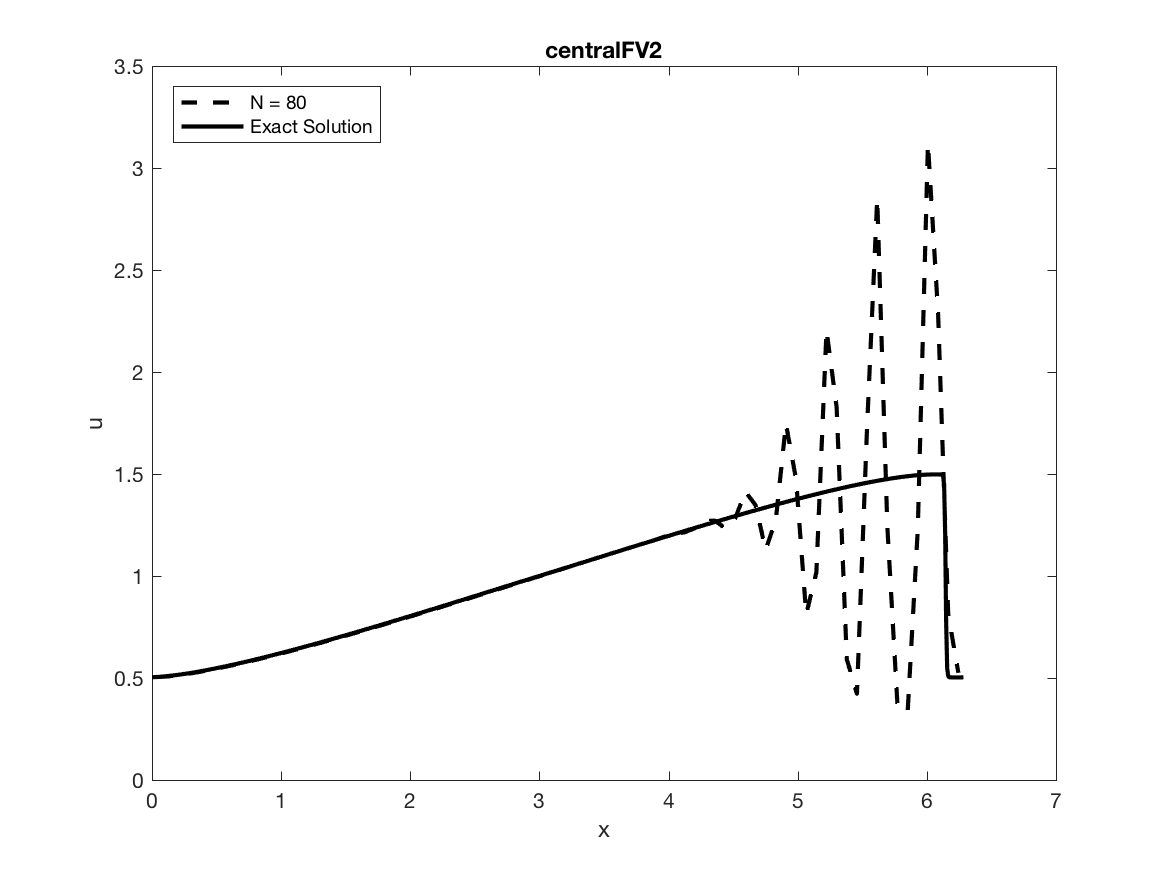
\includegraphics[scale=0.5]{Figures/06_01.png}
          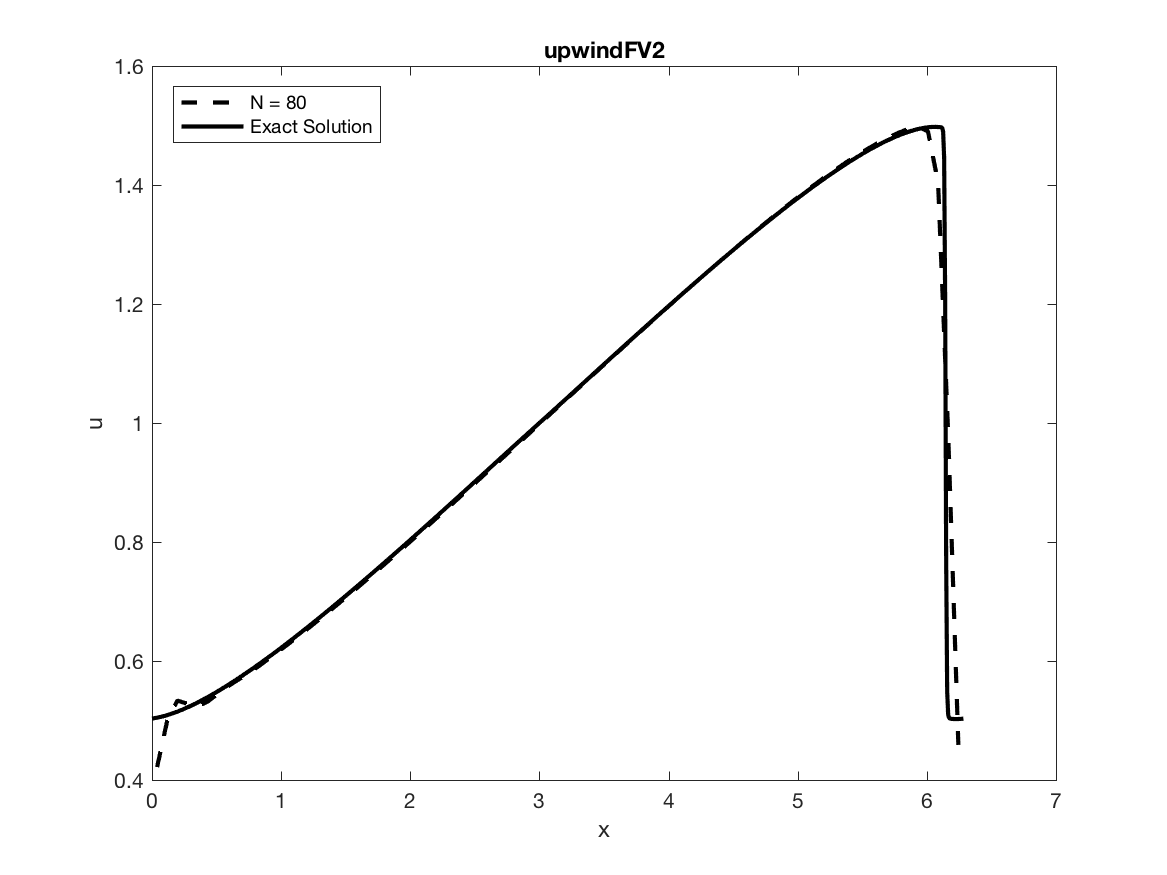
\includegraphics[scale=0.5]{Figures/06_02.png}
          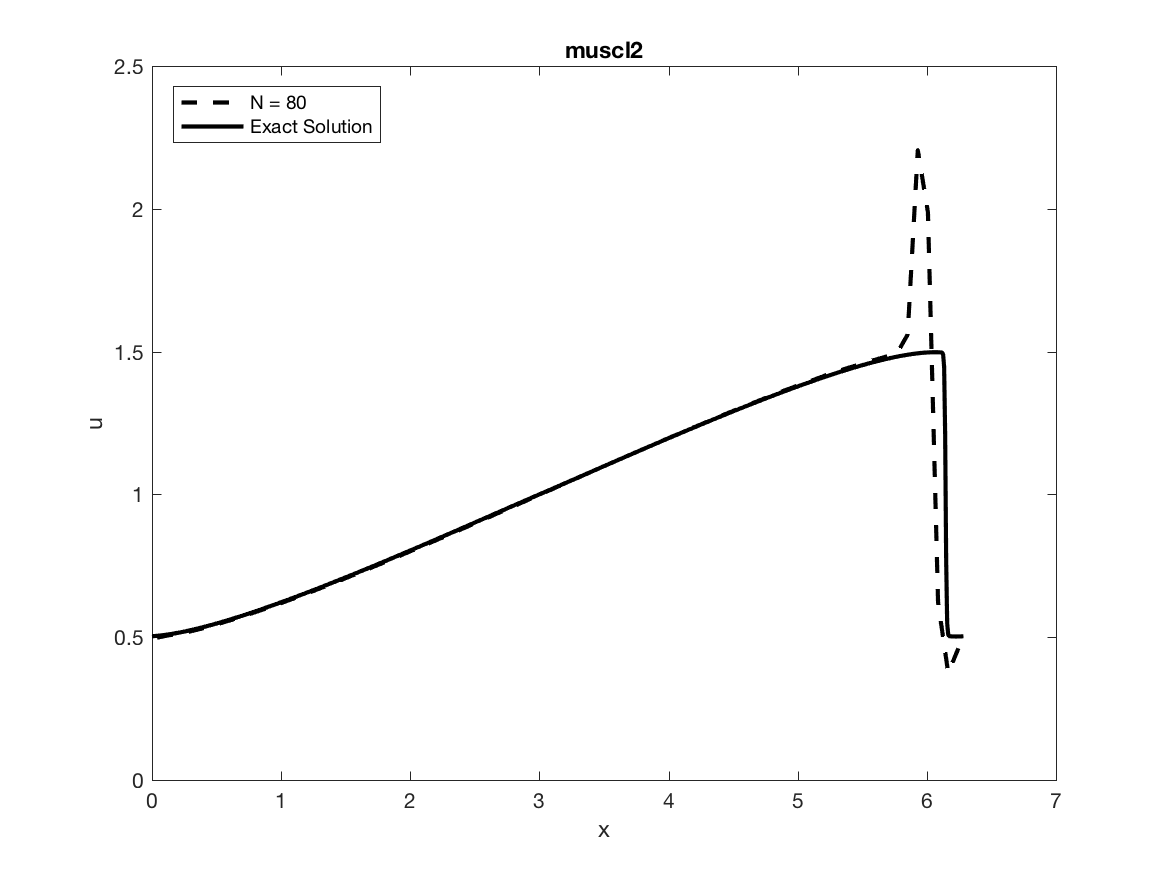
\includegraphics[scale=0.5]{Figures/06_03.png}
        \end{center}
    \end{enumerate}

  \item % #2
    The following script uses the methods from problem 1 on the advection
    equation.
    \lstinputlisting[language=MATLAB, firstline=89]{H06.m}
    The following images are produced.
    Again these are using 2nd order space discretizations without any slope
    limiters, so oscillations occur around discontinuities.
    \begin{center}
      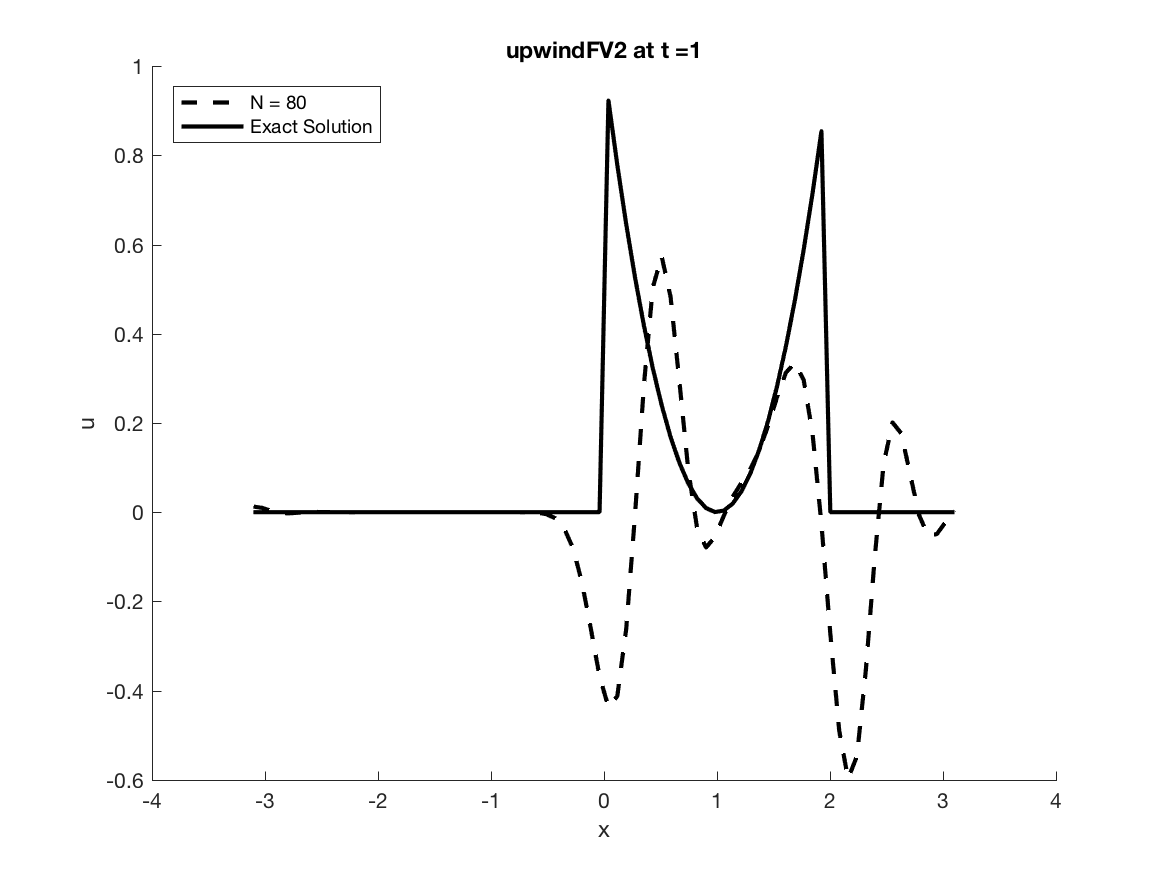
\includegraphics[scale=0.4]{Figures/06_04.png}
      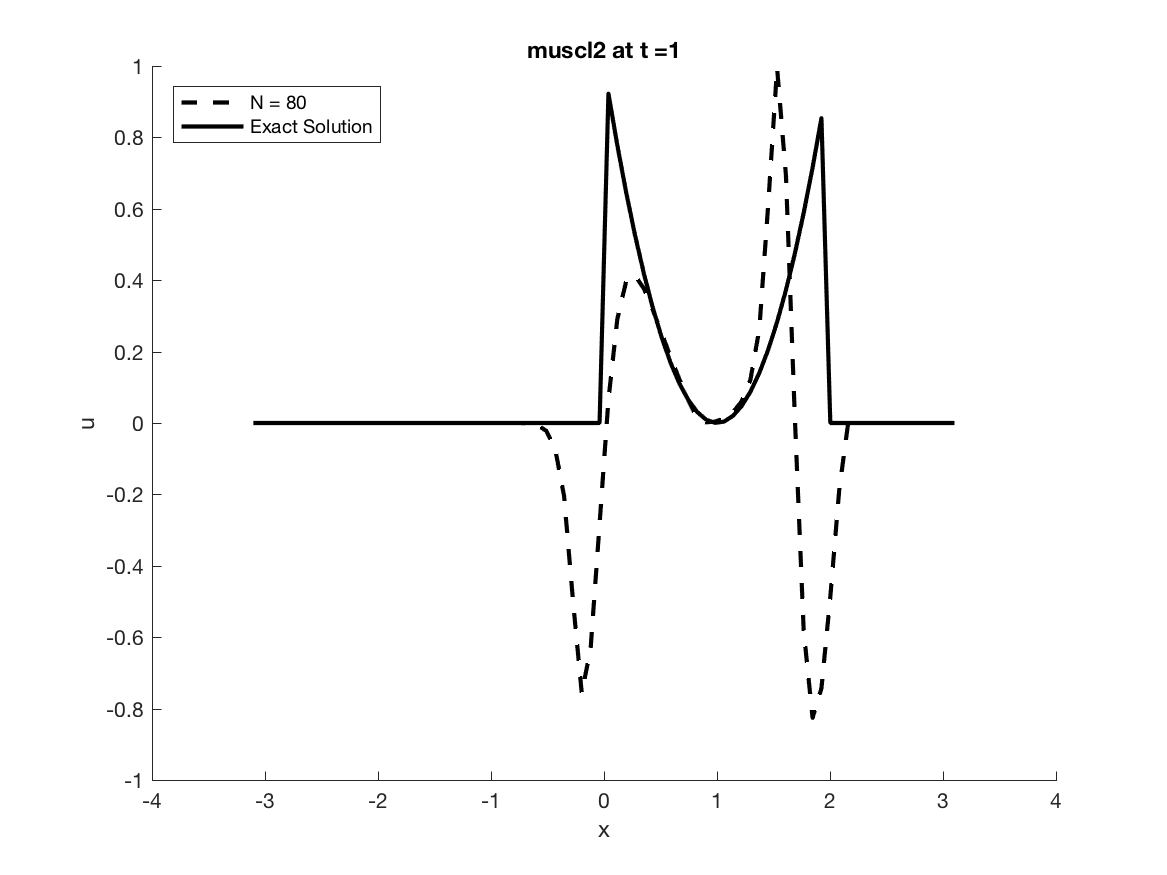
\includegraphics[scale=0.4]{Figures/06_05.png}
      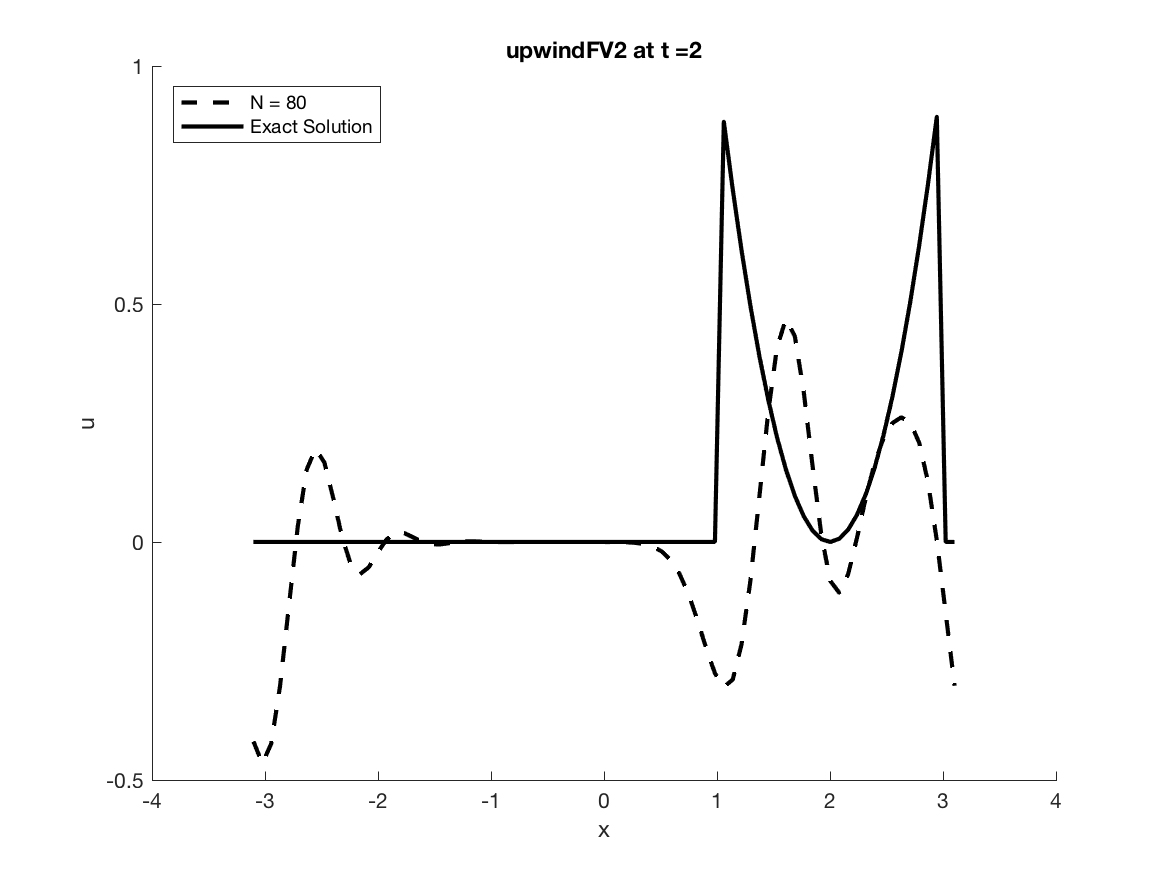
\includegraphics[scale=0.4]{Figures/06_06.png}
      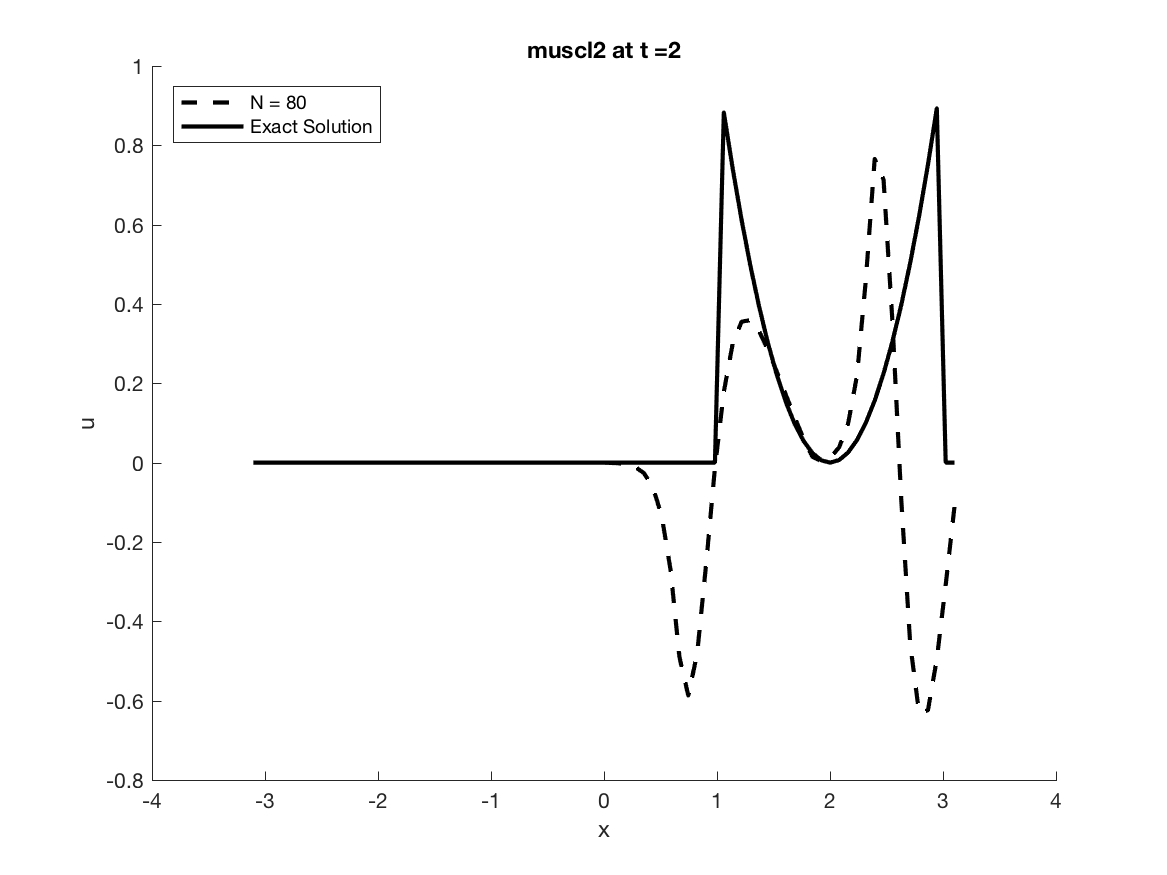
\includegraphics[scale=0.4]{Figures/06_07.png}
    \end{center}

\end{enumerate}
\end{document}
